%% ICSE 2027 NIER. 4 pages main text + 1 page references. Double-anonymous.
%% Compile: pdflatex paper && pdflatex paper   (bibliography is inline; no bibtex pass needed)
%% NOTE: no TeX engine was available where this was written -- compile on Overleaf.
\documentclass[10pt,conference]{IEEEtran}
\IEEEoverridecommandlockouts

\usepackage{cite}
\usepackage{amsmath,amssymb}
\usepackage{graphicx}
\usepackage{booktabs}
\usepackage[hidelinks]{hyperref}
\usepackage{balance}

\begin{document}

\title{Context Is a Pipeline, Not a Window:\\
Information Attrition in LLM Agent Harnesses}

\author{\IEEEauthorblockN{Anonymous Author(s)}
\IEEEauthorblockA{Submitted for double-anonymous review}}

\maketitle

\begin{abstract}
LLM agents are judged by two numbers: how large the context window is, and how
often the final answer is right. Both miss a third thing: how much of a tool's
output is lost before the model ever sees it. We measured this in a tool-using
agent that diagnoses faults from kernel traces. The window was almost empty
--- $6.6\%$ used at the median. Yet a third of all tool results ($3{,}827$ of
$11{,}189$) were cut in transit, and every cut result was broken JSON. The
loss had a pattern. The harness cut results by slicing the JSON text at a
fixed length. A slice like that deletes whatever sits late in the text. One
field reached the model in $4.7\%$ of calls; its neighbour, in the same
results, reached it in $99.3\%$. Which field holds the culprit depends on
whether the culprit process started during the trace --- and the benchmark's
accuracy split matched that line exactly. So we ran controlled experiments to
test whether the cut \emph{caused} the split. This paper contributes: a model
of agent context as a five-stage pipeline, with a way to measure loss at each
stage; replays of $864$ real tool results, including a production trace where
the shipped cut deletes all $128$ records of the culprit's class; an
experiment showing the cut's cost arrives as extra work before it arrives as
errors ($+28\%$ tool calls, double the computations, yield falling
$0.61\rightarrow0.31$), while the answer survives when the agent has other
ways to reach it; and a survey showing that today's agent frameworks cut the
same way. Whether the cut causes the accuracy split is still open. We report
the experiments that failed to settle it.
\end{abstract}

\begin{IEEEkeywords}
LLM agents, agent harnesses, context engineering, empirical evaluation
\end{IEEEkeywords}

\section{Introduction}
\label{sec:intro}

An agent does not read its context window. It reads what its harness --- the
code around the model --- decided to put there. Between a tool producing a
result and the model seeing it, the harness serializes the result, cuts it to
a budget, keeps or trims it across turns, and hands it between agent phases.
Each step is a design choice. Each step can lose information.

Research on agent context mostly asks how big the window is and how the model
attends within it~\cite{liu2024lost}, or how to extend it with
memory~\cite{packer2023memgpt}. Papers about harnesses treat the scaffolding
as a detail~\cite{yang2024sweagent,jimenez2024swebench}. One recent study
reads the source code of eleven production harnesses, but measures no
effects~\cite{harness2026}. Failure taxonomies label what went wrong across
thousands of agent runs~\cite{cemri2025mast}. That last line of work is the
closest to ours, and the gap is simple: \textbf{a run log records what a tool
\emph{delivered}, not what it \emph{produced}}. A loss on the way into the log
cannot be found in the log. No evaluation today reports how much of what an
agent produced survived to its decision.

We measured it, in an agent that finds the root cause of injected faults from
Linux kernel traces. Three facts came out.

First, the window was nearly empty. The largest single prompt in $120$ runs
was $23$k tokens, against a $400$k window. The median run peaked at $6.6\%$.

Second, a third of all tool results were destroyed on the way to the model.
The harness cut long results by slicing the JSON text. JSON keeps its keys in
a fixed order, so the slice does not shorten a result --- it deletes the late
keys whole. One list of containers reached the model in $4.7\%$ of $742$
calls. Its sibling list, in the same payloads, reached it in $99.3\%$.

Third, the damage lined up with the task. A fault process that \emph{starts}
during the trace lands in the early list, which survives. A container that was
\emph{already running} appears only in the late list, which dies. Accuracy
split along exactly that line, on both test applications: faults that spawn a
process scored $40$--$55$ out of $60$; faults in already-running containers
scored $0$--$24$ out of $60$. We had read this as a limit of kernel traces. The
delivery numbers say our own harness played a part. How large a part is the
open question, and we report both what our experiments settled and what they
did not.

Our contributions: (1) a five-stage pipeline model of agent context, with a
measured failure at each stage (Sec.~\ref{sec:pipeline}); (2) a way to measure
the loss --- per-stage counts and a single \emph{yield} number --- applied to
our own harness (Sec.~\ref{sec:ablation}); (3) replay evidence, including the
shipped cut deleting a culprit's whole evidence class on a production-scale
trace (Sec.~\ref{sec:measured}); (4) a registered, controlled experiment whose
result is a \emph{compensation tax}: where the agent has other routes to the
answer, the cut costs work, not accuracy (Sec.~\ref{sec:ablation}); and (5) a
survey of seven agent frameworks showing the same kind of cut is the norm
(Sec.~\ref{sec:measured}).

\section{Context as a Pipeline}
\label{sec:pipeline}

We model the path from tool output to decision as five boundaries
(Table~\ref{tab:pipeline}). No agent can skip them. Every tool-using agent
must serialize results, cut them to some budget, keep or trim them across
turns, and move conclusions between phases. A harness that seems to skip a
stage has picked a default for it.

The loss at a boundary is not random. A cutting rule interacts with the shape
of the data. If results keep a fixed key order and the cut is a prefix slice,
then whether a field survives depends on its \emph{position} in the text.
Nothing makes late fields less important than early ones. Models already
attend unevenly by position inside the window~\cite{liu2024lost}. The harness
adds a harsher version of the same problem: a field past the cut is not
attended to less. It is gone before attention sees it.

\begin{table}[t]
\caption{The five boundaries, and the failure we measured at each one in our
harness. S1 and S4 are measured in this paper's experiments. S2 and S3 come
from the harness's earlier instrumented runs. S5 is a design choice here.}
\label{tab:pipeline}
\centering\small
\begin{tabular}{@{}llp{4.0cm}@{}}
\toprule
& \textbf{Boundary} & \textbf{Measured failure} \\
\midrule
S1 & produce $\to$ deliver & prefix slicing: $34\%$ of results cut, all broken; one field delivered $4.7\%$ vs $99.3\%$ \\
S2 & deliver $\to$ act & the step budget is a wall: $51\%$ of $554$ workers stopped at exactly the limit \\
S3 & act $\to$ retain & re-sending the thread: raising retention $80$k$\to$$150$k chars moved one run $303$k$\to$$545$k tokens \\
S4 & retain $\to$ transfer & hand-off is voluntary: $98$ of $554$ workers passed on nothing; silence reads as ``nothing found'' \\
S5 & transfer $\to$ persist & nothing survives the run (on purpose here, to keep runs independent) \\
\bottomrule
\end{tabular}
\end{table}

\textbf{Measuring the loss.} We propose to instrument these boundaries and
report, next to accuracy, how much produced evidence survived each one. The
units must be concrete. At S1 the unit is a top-level field of a tool result.
It counts as delivered when its content is present in the text the model
receives. Whether the payload still parses is reported separately. At S4 the
unit is a recorded finding or a captured computation. It counts as transferred
when it reaches the phase that decides. Our summary number, \emph{yield}, is
findings recorded divided by computations run. It is a narrow, fully
measurable proxy for ``work that reached the decision.'' It does not measure
relevance; that needs ground truth and is future work.

\section{The Defect, Measured}
\label{sec:measured}

\subsection{In the field}
The numbers above come from the harness's deployed evaluation: $720$ runs,
$11{,}189$ tool results, $3{,}827$ cut, all broken; the $4.7\%$/$99.3\%$ split
over $742$ calls. One note on provenance: the accuracy figures came from the
strict scorer, which checks a claimed container against ground truth. They did
not come from the lenient scorer we later caught, and replaced, in our own
experiment tooling.

\subsection{Mechanism and replays}
\label{sec:e1}

\begin{figure}[t]
\centering
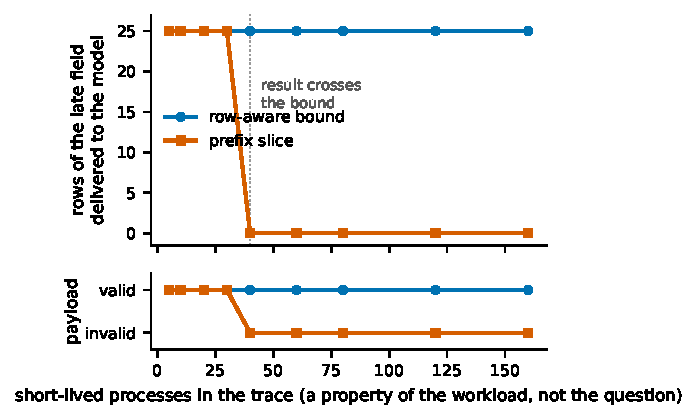
\includegraphics[width=\columnwidth]{fig_cliff.pdf}
\caption{The delivery cliff. We build a result with the real tool's shape and
replay it through both cutting rules. No model is involved. We vary one thing:
how many short-lived processes the trace holds. Under the prefix slice, the
late field arrives whole until the result crosses the budget --- then it
vanishes, and the payload breaks. The row-aware cut keeps every field at every
size.}
\label{fig:cliff}
\end{figure}

The mechanism is deterministic (Fig.~\ref{fig:cliff}). It also holds on real
data. Our transcripts store, for every tool call, both the full result and the
exact text sent to the model. We replayed $864$ recorded results from $31$
runs through both cutting rules. Every result over the budget broke under the
prefix slice: $100\%$. None broke under row-dropping. The tools that overflow
are the ones that \emph{list things}: $50\%$ of process-listing calls broke,
$43\%$ of the agent's own analysis outputs, $1\%$ of small summaries. Only
$2.5\%$ of all calls were affected at all. That is why a defect like this
survives inspection. It is quiet on most calls and fatal on the ones that
matter.

We then replayed the shipped cut on a production-scale trace: a real
$21$-container deployment with one service held under a CPU limit. The culprit
here is quiet. It was already running, and it is one Java container among
five, each near $1.4\%$ of kernel events. The listing result is $33{,}370$
characters --- $5.6\times$ the shipped budget, so nothing is calibrated. The
shipped slice delivers $30$ of $118$ early-list records and \textbf{$0$ of
$128$} late-list records, in a broken payload. On the deployed data, at the
deployed budget, the culprit's whole evidence class disappears before the
model sees it.

\subsection{The same cut in other frameworks}
We read the tool-output cutting code in current releases of seven agent
frameworks (langchain-core 1.6.12, langchain 1.4.6, smolagents 1.26.0,
openai-agents 0.24.0, autogen-agentchat 0.7.5, pyautogen 0.10.0, crewai
0.11.2). Both general-purpose cutters we found slice by position.
langchain-core slices serialized tool output to $500$ characters, keeping the
front. smolagents deletes the \emph{middle} of any observation over $20$k
characters. Neither looks at the structure of what it cuts. Three frameworks
cut nothing, which pushes the loss to the window instead. One cuts only
tracing data. The one structure-aware cutter we found --- a shell middleware
that cuts by lines and says so --- shows the safe pattern exists. It is just
not the default.

\section{The Controlled Experiment}
\label{sec:ablation}

The field numbers show a match, not a cause. And the original repair shipped
together with new tools, so its effect cannot be separated. So we put each
defect back on its own, holding everything else fixed. We wrote down our
predictions before each wave of runs. Every change to the plan is logged, with
its date and reason, in a file that ships with the artifact.

\textbf{Setup.} The subjects are kernel traces of a coding agent running under
resource limits, with exact ground truth. The diagnosing agent, model
(temperature $0$), tools, and task stay fixed. Two fault classes:
\emph{spawned} (the culprit process starts mid-trace) and \emph{resident} (it
was already running). Healthy traces are the negative controls. Every run gets
the same one-line symptom report. The configurations: \emph{repaired}
(row-aware cut, automatic hand-off), \emph{S1 defect} (prefix slice, at the
budget that actually bites on these traces), \emph{S1 reversed} (same defect,
but the keys are serialized in reverse order --- same content, only positions
move), an \emph{order-only} control (reversed keys, no cut), single-defect
arms for S2--S4, and \emph{all defects}. Each class has $5$ distinct
recordings $\times$ $3$ repeats, paired across configurations. $145$ runs; none
failed. Scoring counts only a \emph{commitment}: the agent must name the
culprit in its answer field, and we check the name against ground truth. A
mention in passing does not count. Our first scorer counted mentions. It
inflated one arm from $2/15$ to $14/15$. We caught it by auditing at $46$ runs
and replaced it.

\begin{table}[t]
\caption{The experiments at a glance.}
\label{tab:map}
\centering\small
\begin{tabular}{@{}lll@{}}
\toprule
\textbf{Dataset} & \textbf{n} & \textbf{Used for} \\
\midrule
deployed evaluation & $720$ runs / $11{,}189$ results & S1 field rates \\
worker campaigns & $554$ workers & S2, S4 field rates \\
replay corpus & $31$ runs / $864$ results & cutting-rule replays \\
production trace & $1$ run / $246$ records & shipped-budget replay \\
this experiment & $145$ runs & Table~\ref{tab:compensation} \\
probe runs & $3$ runs & resident baseline check \\
\bottomrule
\end{tabular}
\end{table}

\begin{table}[t]
\caption{The cut changes the price, not the answer. Medians over the $15$
spawned-culprit runs per configuration ($5$ recordings $\times$ $3$ repeats;
order-only has $10$). Yield = findings recorded $\div$ computations run.}
\label{tab:compensation}
\centering\small
\begin{tabular}{@{}lrrrrrr@{}}
\toprule
 & \textbf{correct} & \textbf{calls} & \textbf{cut/run} & \textbf{comp.} & \textbf{yield} & \textbf{tokens} \\
\midrule
repaired         & 14/15 & 53 & 0  & 18 & 0.61 & (567k) \\
S1 defect        & 15/15 & 68 & 27 & 32 & 0.34 & $+5\%$ \\
S1 reversed      & 15/15 & 76 & 30 & 36 & 0.31 & $+14\%$ \\
order only       & 10/10 & 48 & 0  & 16 & 0.61 & $-12\%$ \\
\bottomrule
\end{tabular}
\end{table}

\textbf{Results} (Table~\ref{tab:compensation}). The window was never the
limit. A run used a median $567$k input tokens in total, spread over a median
$53$ calls --- about $10$k per call, against a $400$k window. Under the defect
the agent lost a median $27$ results per run, $40\%$ of its calls, every one
broken. It still named the spawned culprit in $15/15$ runs, against $14/15$
repaired. That difference is noise at this sample size. It does not mean the
defect helps. What moved was the work. Tool calls went $53\to68\to76$
($+28\%$, $+43\%$). Computations went $18\to32\to36$ --- about double. Input
tokens went up $5\%$, then $14\%$. Yield fell $0.61\to0.34\to0.31$. The yield
falls because wasted production grows, not because findings drop --- findings
stay at $11$ throughout. The order-only control lands back at exactly $0.61$,
which also checks the metric itself. At equal answers, the extra tokens are
pure waste: an energy cost that no latency metric will ever show.

\textbf{The reversal test, and a refuted prediction.} We registered a
prediction: reversing the key order moves the culprit's list from fully
delivered to fully deleted, so accuracy should drop. The manipulation worked.
The transcripts show the culprit absent from every listing payload. The agent
still named it, $15/15$. It recovered the name through its own code: the
culprit is the loudest process in the trace ($14.0\%$ of kernel events), so
every sorted table the agent builds puts it in the first rows, inside the part
that survives. The order-only control was flat, so this recovery is real, not
an artifact. What replaces the prediction is a sharper rule:
\textbf{the cut hurts only where the agent has no second route to the answer,
and its cost shows up as work before it shows up as errors.} A loud culprit
survives the loss of any single route. A quiet culprit that lives in one field
--- the resident case in the field data, delivered at $4.7\%$ --- has no
second route.

\textbf{Two predictions we could not test.} H3 said: removing the S4 hand-off
channel turns failures into confident ``nothing is wrong'' answers. But the
repaired baseline already answers ``normal'' on $14/15$ resident runs, so
there is no room to show a shift. H4 said: yield predicts accuracy better than
window use does. But accuracy barely varies inside each class, so no predictor
comparison is possible here. Both stay registered and untested. The S4 worry
itself is grounded in the field data: one worker computed the deciding rate
--- $1{,}242.8$ per second falling to $0$ --- passed on nothing, and the run
concluded ``normal.''

\textbf{Three failed attempts at the causal link.} We tried to show the cut
destroying \emph{accuracy}, not just data, on the production trace from
Sec.~\ref{sec:e1}. The repaired agent failed there too. Plain, or given the
written procedure for this fault, it could not name the throttled service,
and twice named the database one step behind it. With no working baseline
there is nothing for the defect to break, so we did not run that matrix.
The honest summary: the data-destruction half is proven; the accuracy half is
still a correlation. The field split was plausibly caused by agent limits and
delivery loss together. The causal accuracy experiment, on a fault family
where the repaired agent is known to work, is our first item of future work.

\section{Why Nobody Notices}
\label{sec:unnoticed}

Three things hide this class of defect. First, it costs almost no time. In
kernel traces of two production coding agents ($10$ uncapped runs, median
$84\%$, range $80$--$91\%$, network and queueing included), the wall clock is
dominated by waiting for the model. The defect's costs --- correctness and
tokens --- barely touch the metric teams watch. Second, capacity looks fine. A
window at $6.6\%$ use gives no hint that evidence is being discarded. Third,
the usual remedy hides the symptom. In this system, handing the agent a
written procedure reached the same verdict as free exploration at $35\%$ of
the tokens. Teams that feel context pressure add structure, see improvement,
and stop looking. It is the right fix for the wrong reason: it needs less
delivered evidence, instead of delivering evidence better.

\section{Threats to Validity}

One harness, one domain, one model. We argue the defect class is general
because the pipeline is unavoidable and because position-based cutting is what
current frameworks ship (Sec.~\ref{sec:measured}). We have not measured other
harnesses end to end. We also wrote the defect ourselves; that is why the
experiment reintroduces it under registered predictions instead of telling a
repair story. Scale: $5$ recordings per class, with paired repeats; the
experiment's budget is scaled to its smaller traces, while the
production-scale replay uses the shipped budget unchanged. And as stated
above: the accuracy half of the field split remains correlation, not cause.

\section{Future Plans}

\textbf{(1) The causal accuracy experiment.} Pick a fault family where the
repaired agent is known to succeed and the culprit is quiet. Reverse the key
order, and nothing else. For every run, report four checks: culprit records
visible to the model, payload valid or broken, culprit recoverable by other
tools, and the final answer. \textbf{(2) A deeper survey.} Extend our reading
of seven frameworks across the eleven-harness corpus of~\cite{harness2026}.
Classify every cutter as position-based or structure-based, and run each one
against the delivery-cliff replay. \textbf{(3) Reporting loss as standard
practice.} Package the instrument so any harness can print its loss profile
next to its accuracy number. The claim to test: harnesses with equal accuracy
differ in yield, and yield predicts how they do on harder tasks. \textbf{(4)
Tests without a model.} Each failure in Table~\ref{tab:pipeline} is mechanical,
so CI can catch it: a result that does not survive its own cut, a step budget
with a pile-up at its limit, a phase boundary that drops computed results. A
replication package (drivers, scorer, per-run results, replay corpus, and the
registered plan with its dated amendment log) is prepared for artifact
submission.

\section{Conclusion}

An agent's context is not a window it is given. It is the output of a pipeline
its harness built. In a working system, that pipeline destroyed a third of all
tool results while the window sat $93\%$ empty. It deleted evidence by
position, not by value. Where the agent had another route to the answer, the
loss turned into measurable extra work instead of errors. Every harness makes
these choices. None reports them. They are easy to measure, and we have shown
how.

\balance

\begin{thebibliography}{9}
\bibitem{liu2024lost}
N.~F. Liu, K.~Lin, J.~Hewitt, A.~Paranjape, M.~Bevilacqua, F.~Petroni, and
P.~Liang, ``Lost in the middle: How language models use long contexts,''
\emph{Transactions of the Association for Computational Linguistics}, vol.~12,
pp.~157--173, 2024.

\bibitem{packer2023memgpt}
C.~Packer, S.~Wooders, K.~Lin, V.~Fang, S.~G. Patil, I.~Stoica, and J.~E.
Gonzalez, ``{MemGPT}: Towards {LLMs} as operating systems,'' \emph{arXiv
preprint arXiv:2310.08560}, 2023.

\bibitem{yang2024sweagent}
J.~Yang, C.~E. Jimenez, A.~Wettig, K.~Lieret, S.~Yao, K.~Narasimhan, and
O.~Press, ``{SWE-agent}: Agent-computer interfaces enable automated software
engineering,'' in \emph{Advances in Neural Information Processing Systems
(NeurIPS)}, 2024.

\bibitem{jimenez2024swebench}
C.~E. Jimenez, J.~Yang, A.~Wettig, S.~Yao, K.~Pei, O.~Press, and
K.~Narasimhan, ``{SWE-bench}: Can language models resolve real-world {GitHub}
issues?'' in \emph{International Conference on Learning Representations
(ICLR)}, 2024.

\bibitem{cemri2025mast}
M.~Cemri, M.~Z. Pan, S.~Yang, L.~A. Agrawal, B.~Chopra, R.~Tiwari,
K.~Keutzer, A.~Parameswaran, D.~Klein, and K.~Ramchandran, ``Why do
multi-agent {LLM} systems fail?'' \emph{arXiv preprint arXiv:2503.13657},
2025.

\bibitem{harness2026}
P.~Barbaste, T.~Darrigol, G.~Vu, and T.~Wiltberger, ``Harness engineering:
Anatomy, architecture, and evolution of coding agents --- a source-code study
of eleven systems,'' \emph{arXiv preprint arXiv:2609.00006}, 2026.
\end{thebibliography}

\end{document}
